\subsection{Setzeinheit} \label{sec:Inbetriebnahme_Setzeinheit}
\textit{(pro)} Ähnlich wie ION Motion bietet auch Trinamic eine eigene PC Software für die Ansteuerung ihrer Motorencontroller an. Trinamic nennt das Tool dabei TMCL-IDE. Die TMCL-IDE wurde für eine ganze Familie von Motorencontroller entwickelt. Diese Software ist sehr umfangreich und bietet Tools zur Identifikation des verwendeten Motors sowie dessen Hall Sensoren, zur Bestimmung von Regelparameter, Programmierung von Bewegungsabläufen und vielem mehr. In Abb. \ref{fig:TMCL-IDE} ist ein Auszug der Software zu sehen.

\begin{figure}[H]
	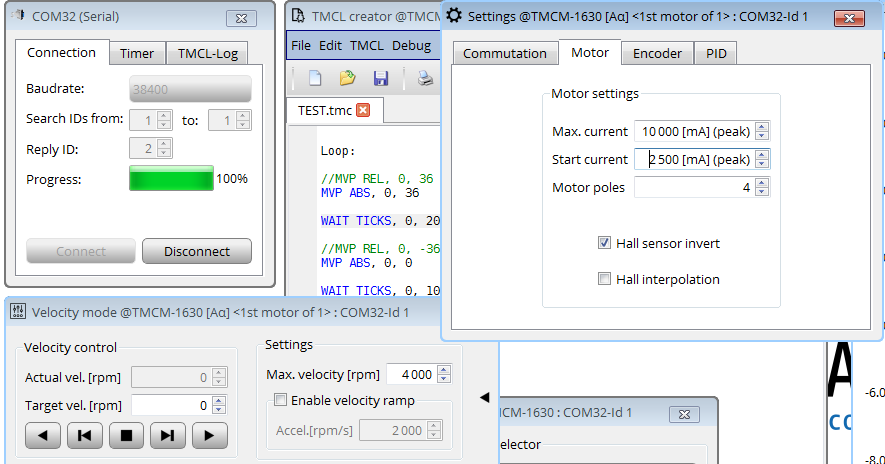
\includegraphics[width=0.7\textwidth]{Illustrationen/7-Inbetriebnahme_und_Kalibration/TMCL_IDE.png}
	\caption{Trinamic TMCL IDE}
	\label{fig:TMCL-IDE}
\end{figure}

Im Umfang dieses Projekts wurde mit Hilfe dieser Software der Bewegungsablauf der Setzeinheit eingestellt und durch Verändern der Regelparameter zu einer flüssigen Bewegung optimiert. Für eine optimale Auslastung der Hardware hätte in diesem Teil der Inbetriebnahme noch mehr Zeit investiert werden sollen. Der getestete Bewegungsablauf wurde anschliessend auf die Software des FRDM-Boards adaptiert. Weiter wurde auch die Initialisierungphase erfolgreich getestet, bei der die Setzeinheit an den oberen Anschlag fährt.

Die Setzeinheit ist fähig die Stechbewegung deutlich unter einer Sekunde zu absolvieren. Aufgrund der fehlenden Zeit können keine quantitative Aussagen gemacht werden. Auch konnte das Ausheben eines Setzloches nicht getestet werden.

\subsection{Stechdorn}
\textit{(ygu)} Der entwickelte Stechdorn konnte mit dem vorgesehenen Spielmass montiert werden (vgl. Kap. \ref{spitzeoben}). Die Montage erfolgte erfolgreich, nur wenig Material musste von der Deckschicht abgetragen werden. Im Einsatz funktioniert der Stechdorn, wie folgt:
\begin{figure}[H]
	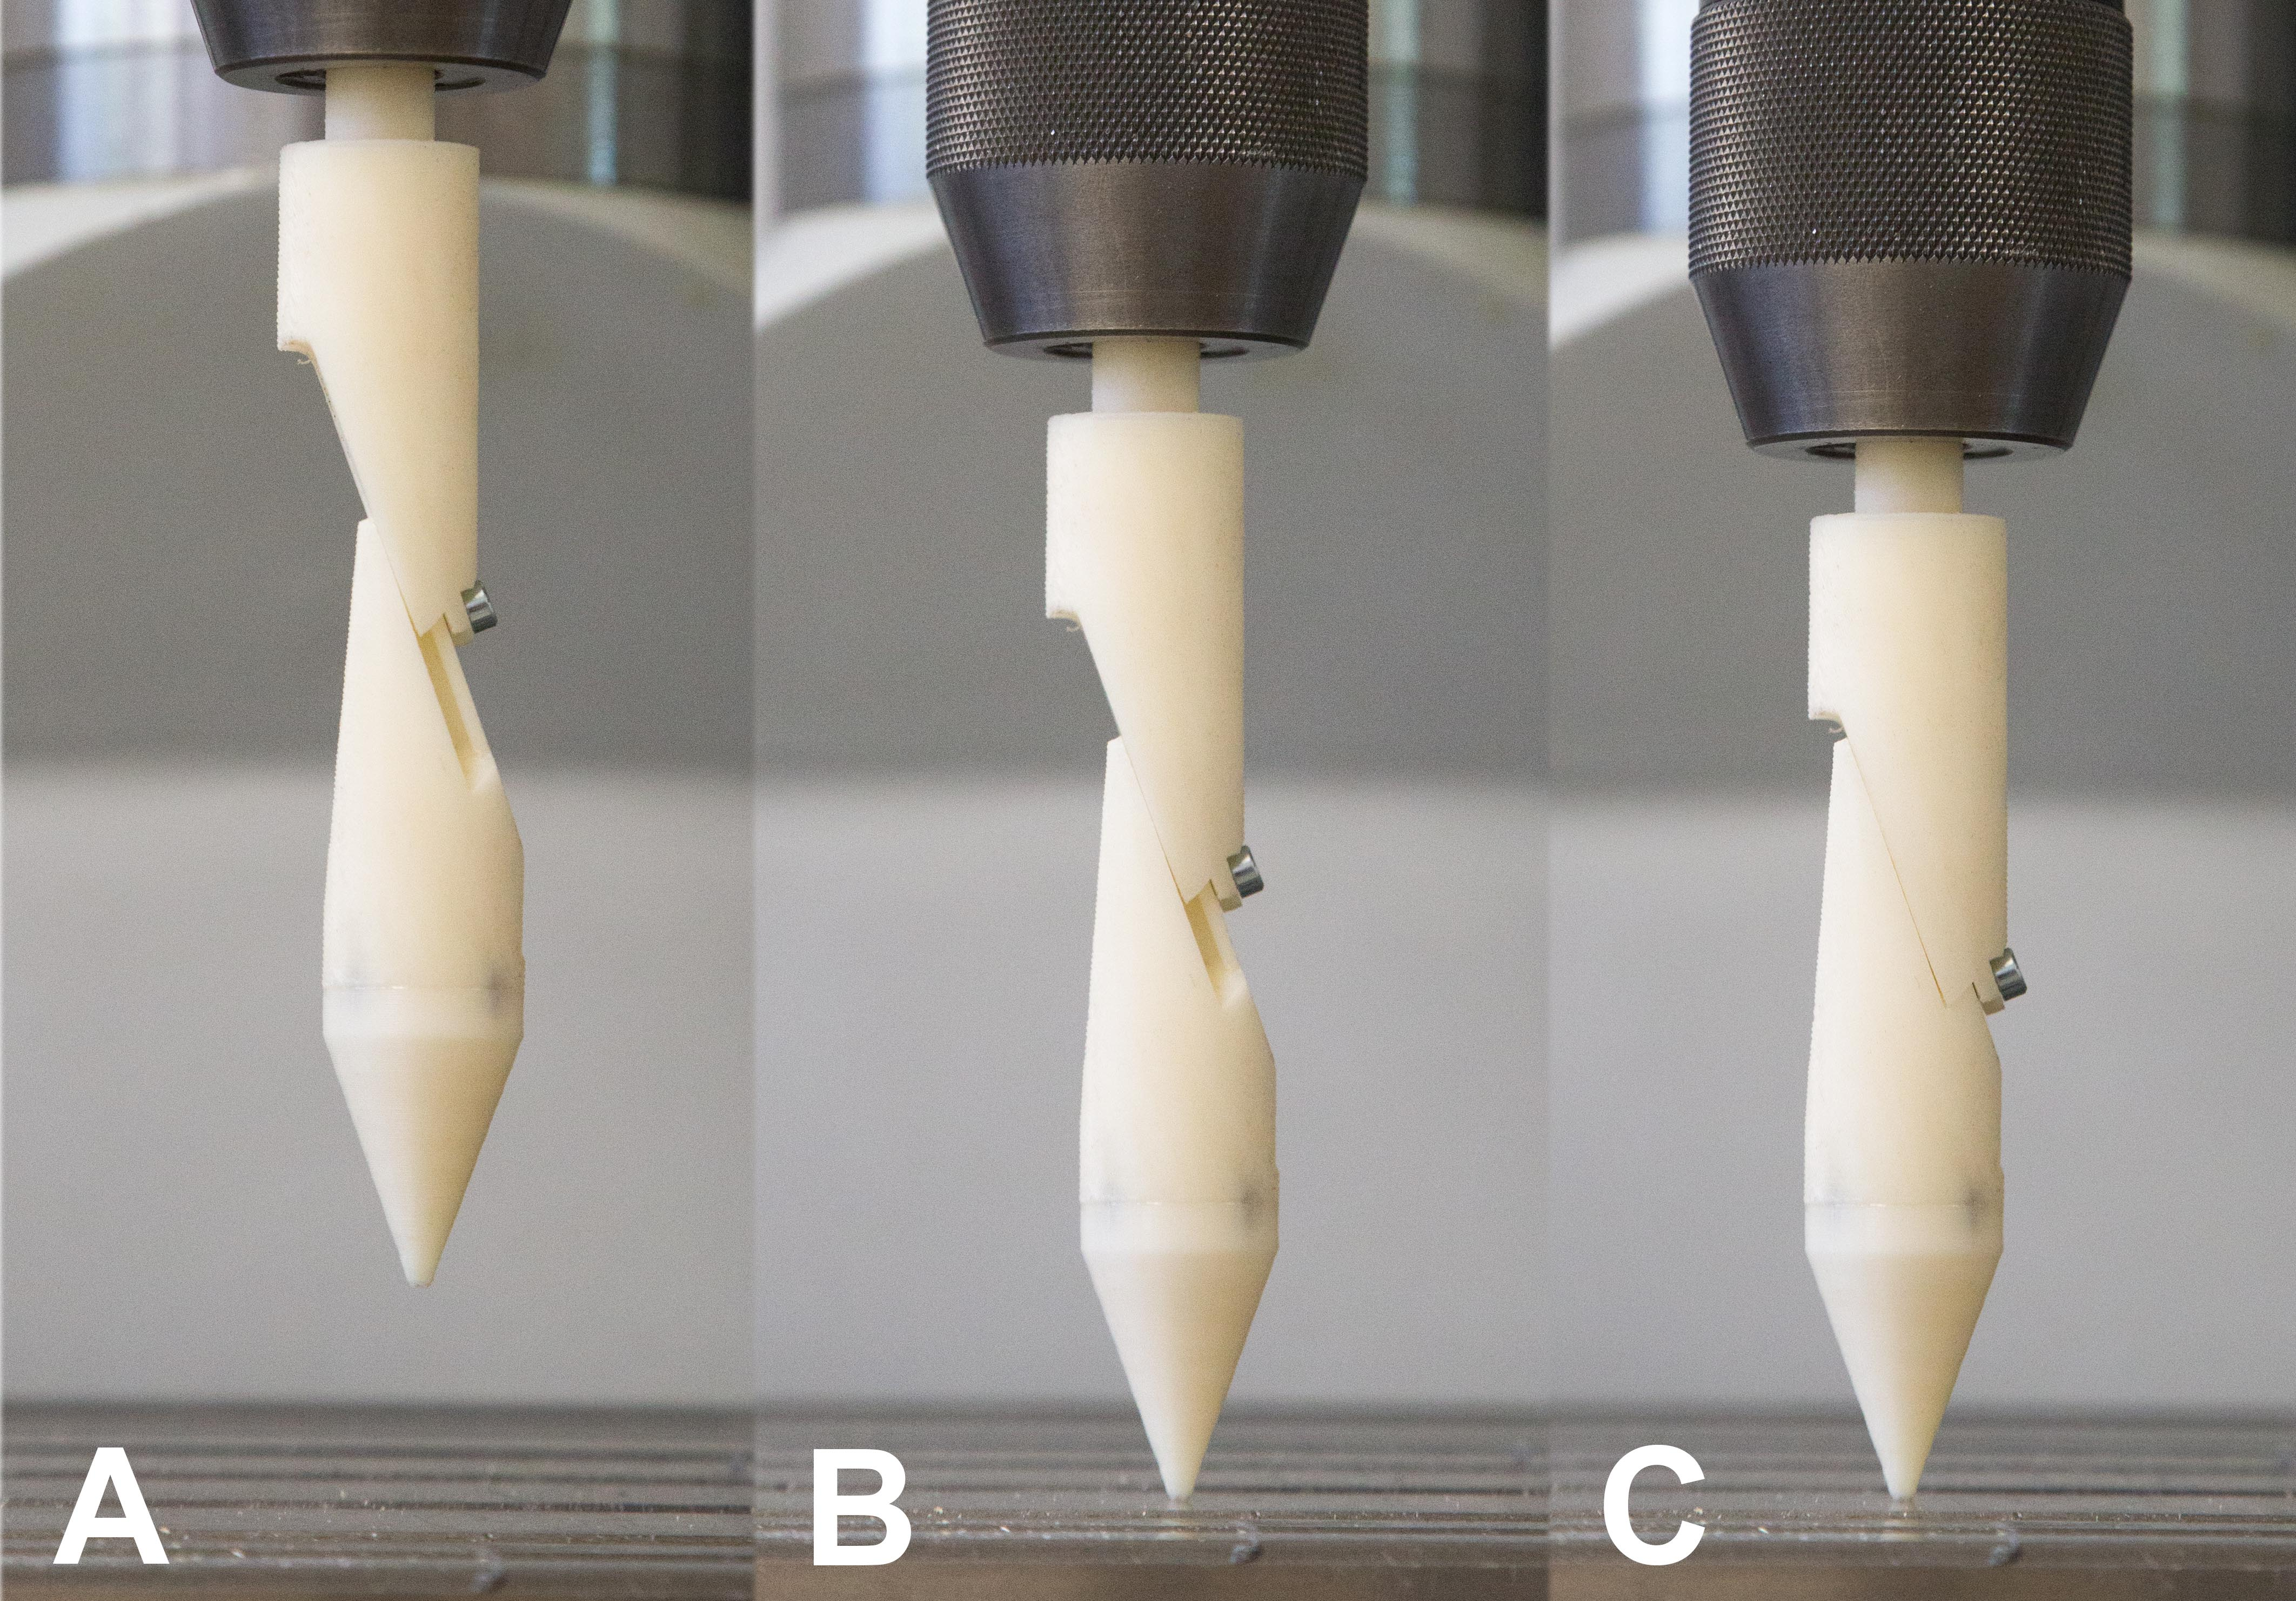
\includegraphics[draft=false,width=0.7\textwidth]{Illustrationen/7-Inbetriebnahme_und_Kalibration/inbet_stechdorn.jpg}
	\caption{Schliessvorgang des Stechdorns}
	\label{fig:inbet_stechdorn}
\end{figure}
In Abbildung \ref{fig:inbet_stechdorn} ist ersichtlich, dass der Stechdorn die Schliessbewegung erfolgreich ausführt. Auch öffnet sich der untere Teil durch die Gewichtskraft problemlos.
\newline

Der Stechdorn funktioniert einzeln einwandfrei. Der definitive Nachweis der Funktionalität kann nur im Zusammenspiel mit der Setzeinheit erfolgen.